%!TEX program=lualatex

\def\LectureName/{General Physics I}
%\def\LectureNumber/{}
%\def\LectureDate/{}
\PassOptionsToPackage{fleqn}{amsmath}
\PassOptionsToPackage{hyperfootnotes=false}{hyperref}
\documentclass[11pt,pdfa,lastpage]{MishoNote}
\title{General Physics I: Vector Boot Camp}
\author{Sho Iwamoto}
\hypersetup{
  pdflang={en-US},
  pdfauthortitle={Assistant Professor, National Sun Yat-sen University},
  pdfsubject={Vector Boot Camp (Basic) as a preparation to General Physics 1 lecture.},
  pdfcontactemail={iwamoto@g-mail.nsysu.edu.tw},
  pdfcontacturl={https://www2.nsysu.edu.tw/iwamoto/},
  pdfcaptionwriter={Sho Iwamoto},
  pdfcopyright={2024 Sho Iwamoto\textLF This document is licensed under the Creative Commons CC BY–NC 4.0 International Public License.},
  pdflicenseurl={https://creativecommons.org/licenses/by-nc/4.0/},
}

\usepackage{GP}
\usepackage{pgfornament}
\setlist{itemsep=4pt}
\def\thesection{B}

\newcommand\hrefFN[2]{\href{#1}{#2}\footnote{\url{#1}}}
\newcommand\starskip{\bigskip\begin{center}\pgfornament[width=7cm]{88}\end{center}\medskip}
\newcommand\fakebullet{\makebox[2.5em][r]{\textbullet\kern.5em}}
\makeatletter
\RenewDocumentCommand\new@problem{mm}{%
  \stepcounter{Problem}\item[\kern-2em\kern-\labelsep{\makebox[4.5em][r]{%
        \IfValueTF{#2}{\csname G#2\endcsname}{}{\sffamily\bfseries[\Alph{Problem}]}}}]\relax}
\def\head@j{\color{red}{Work-In-Progress: \mydate\today~\currenttime}}
\makeatother

\let\origfootnote\footnote
\let\origfootnoterule\footnoterule

\begin{document}%
\title{Vector Boot Camp}
\begin{maketitle}
\let\footnote\origfootnote
\let\footnoterule\origfootnoterule

\subsection*{Preface}
Welcome to your first year of university!
As a university student in engineering, \Emph{you must be able to calculate derivatives of ``simple'' functions} such as
\[
\diff{}{x}\frac{x^2+\tan x}{\sin(2x+1)}.
\]
This Boot Camp is designed to help you prepare for your first year, which is unexpectedly tough for most of you!
Take your time, go through each problem carefully, and don't hesitate to ask for help!

To motivate you, we will have a \Emph{mini test} at the beginning of the second lecture; the problems will be from this Boot Camp.
I hope this preparation will make your university life easier, more enjoyable, and more satisfactory. Good luck!

\paragraph{Background}
While Sho heard that vectors are covered in \JA{高中}, it seems that most of you have not practiced enough and do not have experience enough to proceed to Chapter 7--8.
However, we do not have time to do it in the lecture hours (it will consume 1.5 week).
So, Sho has to ask you to do this exercise \Emph*{before Nov.~1}.
This is \Emph*{critical} for you, so a large point (4.0 points) are given as a reward.



To motivate you, we will have a \Emph{mini test} at the beginning of the second lecture; the problems will be from this Boot Camp.
I hope this preparation will make your university life easier, more enjoyable, and more satisfactory. Good luck!

\subsection*{Remarks}
Sho never provides you with solutions. \Emph{You students} need to make the solution. To this end,
\begin{miniitemize}
  \item Use online resources such as \hrefFN{https://www.wolframalpha.com/}{Wolfram Alpha}.
  \item Share your answers to other colleagues, using LINE or \hrefFN{https://docs.google.com/}{Google Docs}. Compare your answers with theirs.
  \item Ask questions to colleagues, to the TA, or to Sho. You can utilize Sho's \hrefFN{https://www2.nsysu.edu.tw/iwamoto/}{office hours}.
\end{miniitemize}


\enlargethispage{-5em}

\makeatletter
\begin{tikzpicture}[remember picture,overlay]
  \begingroup
  \fontsize{9}{13}\selectfont
    \node[xshift=\@total@leftsep,yshift=25.5mm,anchor=south west,align=left,text width=\textwidth] at (current page.south west) {%
      \href{https://creativecommons.org/licenses/by-nc/4.0/}{
\includegraphics[width=2.2cm]{../figs/by-nc.pdf}}\\[.4em]
      \noindent\textsf{\color{gray}%
      Visit \url{https://github.com/misho104/LecturePublic} for further information, updates, and to report issues.}\par
    };
    \node[xshift=-\@total@leftsep+26mm,yshift=32mm,align=left,text width=\textwidth,anchor=south east] at (current page.south east) {%
      \noindent\textsf{\color{gray}%
      This document is licensed under
      \href{https://creativecommons.org/licenses/by-nc/4.0/}{the Creative Commons CC--BY--NC 4.0 International Public License.}\\
      You may use this document only if you do in compliance with the license.}\par
    };
  \endgroup
\end{tikzpicture}
\makeatother

\end{maketitle}
\newpage


\newsavebox{\VectorSetA}
 \begin{lrbox}{\VectorSetA}
 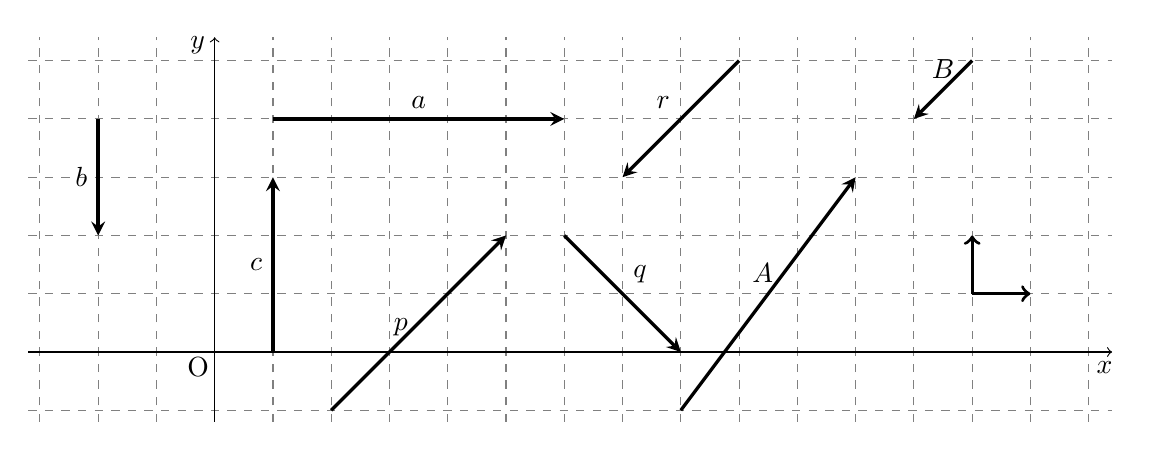
\begin{tikzpicture}[scale=0.74,remember picture]
  \draw[help lines,thin,dashed] (-3.2,-1.2) grid ++(18.6,6.6);
  \draw[->]                     (-3.2,  0 ) --   ++(18.6, 0 ) node[below left,xshift=1.3mm]{$x$};
  \draw[->]                     (  0 ,-1.2) --   ++( 0  ,6.6) node[below left,yshift=1.3mm]{$y$};
  \coordinate (O) at (0,0) node [below left,xshift=.5mm,yshift=.5mm] at (O) {O}; %\fill (O) circle (4pt);
  \draw[-stealth, very thick] (1,4)--node [above]{$\vc a$} ++(5,0);
  \draw[-stealth, very thick] (-2,4)--node [left]{$\vc b$} ++(0,-2);
  \draw[-stealth, very thick] (1, 0)--node [left]{$\vc c$} ++(0,3);
  \draw[-stealth, very thick] (2,-1)--node [above left,yshift=-3mm]{$\vc p$} ++(3,3);
  \draw[-stealth, very thick] (6,2)--node [above right]{$\vc q$} ++(2,-2);
  \draw[-stealth, very thick] (9,5)--node [above left]{$\vc r$} ++(-2,-2);
  \draw[-stealth, very thick] (8,-1)--node [above left,xshift=2mm]{$\vc A$} ++(3,4);
  \draw[-stealth, very thick] (13,5)--node [above]{$\vc B$} ++(-1,-1);
  \draw[->,very thick] (13,1)--node [below]{$\vvex$} ++(1,0);
  \draw[->,very thick] (13,1)--node [left] {$\vvey$} ++(0,1);
  %\fill (O) circle (4pt) (A) circle (4pt) (B) circle (4pt) (C) circle (4pt) (D) circle (4pt);
  \end{tikzpicture}
\end{lrbox}


\subsection{Definition of Vectors}
\begin{definition}{Vectors (for physics)}{def:vec}
\begin{miniitemize}
  \item A vector is a physical quantity that has \Emph{both magnitude and direction}.
  \item We describe them by $\vc a$, $\vc A$, $\vc p\w F$, etc.\addnote{%
    Professionals use boldface, e.g., $\mathbf{a}$, $\mathbf{A}$, $\mathbf{p}\w F$, etc., but in this lecture we only use the beginners' style.},
    and their magnitudes by $|\vc a|$, $|\vc A|$, $|\vc p\w F|$, etc.
  \item We often describe them by arrows. The arrows' direction should match the vector's direction. The arrows' length should be \emph{proportional to} the vector's magnitude.
\end{miniitemize}
\end{definition}
\OutputNote

\begin{definition}{Vector quantity and Scalar quantity}{def:vecsca}
  \begin{miniitemize}
    \item Physical quantities with direction are called \Emph{vector quantity}.
    \begin{miniitemize} \item They can be described by vectors.\addnote{%
      If the space considered is one-dimensional, we can describe the direction by $+$ or $-$ and a vector quantity can be described by a number. Here, however, \Emph{you} must specify which direction is positive.} \end{miniitemize}
    \item Physical quantities without direction are called \Emph{scalar quantity}.
    \begin{miniitemize} \item They can be described by numbers. \end{miniitemize}
    \item Consider a vector quantity $\vc A$. Its magnitude $|\vc A|$ is a scalar quantity.
  \end{miniitemize}
  \end{definition}
\OutputNote
For example, \Emph{mass} $m$ and \Emph{temperature} $T$ are scalar quantities. \Emph{Velocity} $\vc v$ is a vector quantity and its magnitude $|\vc v|$ (it has a special name ``\Emph{speed}'')  is a scalar quantity. Acceleration $\vc a$ is a vector quantity.

\begin{quizzes}
  \Quiz[S] Choose vector quantities. Choose scalar quantities.
  \begin{menumerate}[labelsep=0em,labelwidth=0em,itemindent=1em,label={},leftmargin=0.3em]{4}
    \item temperature
    \item air pressure
    \item wind speed
    \item velocity
    \item electric charge
    \item Sho's height
    \item Sho's weight
    \item Sho's mass
    \item city name
    \item position
    \item time difference
    \item time
    \item duration
    \item distance
    \item kilometer
    \item resistor
    \item resistance
    \item conductor
    \item conductance
    \item conductivity
  \end{menumerate}
\end{quizzes}

\newpage
\subsection{How to describe directions}
\Remark{
  Using natural English is nice, but it is more important, and thus we should pay greater attention, to ensure that the expression is clear and does not cause any misunderstanding.
}
\paragraph{Basic}
\emph{We} need to learn how to describe directions of vectors \Emph{in English}. The easiest one is
\begin{tabbing}
 \fakebullet \= downward   \== toward the bottom      \=\kill
 \fakebullet \> leftward   \>= toward the left        \>= to the left\\[\itemsep]
 \fakebullet \> rightward  \>= toward the right       \>= to the right\\[\itemsep]
 \fakebullet \> upward     \>= toward the top         \>= to the top\\[\itemsep]
 \fakebullet \> downward   \>= toward the bottom      \>= to the bottom
% \item forward / backward (if the front and back are obvious, e.g., a car or bicycle)
\end{tabbing}
If you need to describe the third dimension which is perpendicular to the textbook's page or the sheet (or the blackboard), you can use
\begin{tabbing}
  \fakebullet \= out of the \= (sheet | page | blackboard) \= = away from the \= (sheet | page | blackboard)\kill
  \fakebullet \> into   the \> (sheet | page | blackboard) \> = toward    the \> (sheet | page | blackboard)\\[\itemsep]
  \fakebullet \> out of the \> (sheet | page | blackboard) \> = away from the \> (sheet | page | blackboard)
\end{tabbing}
For 2d case, \Emph{once you specify the ``north'' direction,} you can use the following expressions:
\begin{miniitemize}
 \item northward, southward, eastward, westward (= (to | toward) the north, etc.)
 \item northwestward, southwestward, etc. (= (to | toward) the northwest, etc.)
\end{miniitemize}

\paragraph{With axes}
Usually, we define $x$-axis and $y$-axis (and $z$-axis, if 3d). \Emph{If such axes are defined} (or once you have defined them), we can use
\begin{tabbing}
  \fakebullet \= in the negative $x$-direction \== in the $-x$ direction\kill
  \fakebullet \> in the positive $x$-direction \>= in the $+x$ direction\\[\itemsep]
  \fakebullet \> in the positive $y$-direction \>= in the $+y$ direction\\[\itemsep]
  \fakebullet \> in the negative $x$-direction \>= in the $-x$ direction\\[\itemsep]
  \fakebullet \> in the negative $y$-direction \>= in the $-y$ direction
 \end{tabbing}
In particular, for 2d cases, we can use the angle from the positive $x$-axis (counterclockwise):
 \begin{miniitemize}
  \item $30^\circ$ from the $+x$ axis (= $30^\circ$ counterclockwise from the positive $x$-axis)
  \item $90^\circ$ from the $+x$ axis (= in the $+y$ direction)
  \item $170^\circ$ from the $+x$ axis (= $10^\circ$ clockwise from the negative $x$-axis)
  \item $-15^\circ$ from the $+x$ axis (= $15^\circ$ clockwise from the positive $x$-axis)
  \item angle $\theta$ from the $+x$ axis, where $\tan\theta=0.1$ and $0<\theta<\pi/2$.
 \end{miniitemize}
Sometimes the word ``the horizontal'' is useful:
\begin{miniitemize}
  \item $10^\circ$ above the horizontal / $30^\circ$ below the horizontal
\end{miniitemize}
\Remark{It is difficult to describe general 3d directions by words. For this purpose, we usually use mathematical expressions (i.e., vectors).}

\paragraph{Rotations}
To describe the direction of rotation, we use
\begin{miniitemize}
  \item clockwise / counterclockwise
\end{miniitemize}
If you have an arrow and discuss rotations about the arrow, you can use the following expressions:
\begin{miniitemize}
  \item following the right-hand rule (= counterclockwise when viewed from the arrow's direction)
  \item following the left-hand rule (= clockwise when viewed from the arrow's direction)
\end{miniitemize}
We will often use these expressions in General Physics 2.

\newpage

\subsection{Vectors: Magnitude and Direction}
In this Boot Camp, we forget about physics\addnote{%
 We forget units and significant figures, which you will learn in the beginning of General~Physics~1 lectures. In other words, in the lectures, \Emph{you must not forget units and significant figures} of vector quantities.
}.
Focusing on mathematics, we will discuss vectors in its mathematical aspects.
We will begin with a few more expressions useful for vectors.

If the angle between $\vc a$ and $\vc b$ is $90^\circ$, we say
\begin{tabbing}
  \fakebullet \= \kern16em \=\kill
  \fakebullet \> $\vc a$ is \Emph{perpendicular to} $\vc b$. \> \fakebullet $\vc a$ and $\vc b$ are perpendicular to each other.\\[\itemsep]
  \fakebullet \> $\vc a$ is orthogonal to $\vc b$.   \>    \fakebullet $\vc a$ and $\vc b$ are orthogonal  to each other.\\[\itemsep]
  \fakebullet \> $\vc a$ is normal to $\vc b$.       \>    \fakebullet $\vc a$ and $\vc b$ are normal to each other.
 \end{tabbing}
(all of them are correct but the first one is the most common). If the angle is $0^\circ$, we say\addnote{%
\Emph{Avoid} the word ``parallel'' because some people think it includes both $0^\circ$ and $180^\circ$ cases. Clarity is important in science.}
\begin{tabbing}
  \fakebullet \= \kern16em \=\kill
  \fakebullet \> $\vc a$ is \Emph{in the same direction as} $\vc b$. \> \fakebullet $\vc a$ and $\vc b$ are in the same direction.
\end{tabbing}
Finally, if the angle is $180^\circ$,
\begin{tabbing}
  \fakebullet \= \kern16em \=\kill
  \fakebullet \> $\vc a$ is \Emph{anti-parallel to} $\vc b$. \> \fakebullet $\vc a$ and $\vc b$ are anti-parallel.\\[\itemsep]
  \fakebullet \> $\vc a$ is opposite to $\vc b$.      \> \fakebullet $\vc a$ and $\vc b$ are in opposite directions.
\end{tabbing}

\OutputNote



\begin{problems}
 \Problem[S] Vectors are drawn on the grid, which has a spacing of 1. Answer the following questions.
 \par\smallskip\par\usebox{\VectorSetA}

\begin{enumerate}
  \item Describe the direction (in English words) and magnitude of each vector. Try to use multiple expressions.
  \item Describe relationship between the directions of the following vector pairs:\\
   ($\vc a$ and $\vc b$), ($\vc b$ and $\vc c$), ($\vc p$ and $\vc q$), ($\vc p$ and $\vc r$), ($\vvex$ and $\vvey$), and ($\vc a$ and $\vvex$).\\
   For example, ``$\vc a$ is perpendicular to $\vc b$''.
\end{enumerate}

\end{problems}

\newpage


\subsection{Vector Basics}
These are a few basic things that you have learned in highschool:
\begin{itemize}
\item \Emph*{(Zero vector)} There is a special vector $\vc 0$. Its length is $0$ (zero) and it has no direction.
\item \Emph*{(Scalar multiplication)} If $\vc v$ is a vector, $2\vc v$ and $-3\vc v$ are both vectors.
\item \Emph*{(Addition)} If $\vc p$ and $\vc q$ are vectors, $\vc p + \vc q$ is a vector.
\end{itemize}
By extending the last two items, we can obtain the following statement.
\begin{itemize}
  \item \Emph*{(Linear combination)} If $a$ and $b$ are scalars (i.e., real numbers) and $\vc p$ and $\vc q$ are vectors,
  \[ a\vc p+b\vc q \]
  is a vector. Here, $a$ and $b$ can be positive, zero, or negative.
\end{itemize}

\begin{problems}
 \Problem[S] Vectors are drawn on the grid, which has a spacing of 1.
 \par\smallskip\par\usebox{\VectorSetA}
 \begin{enumerate}
   \item Describe $\vc a$ by using $\vvex$ (and a number).  Describe $\vc b$ and $\vc c$ by using $\vvey$.
   \item Describe $\vc B$ by using $\vc r$. Describe $\vc p$ by using $\vc r$.
   \item Describe $\vc A$ and $\vc B$ by using $\vvex$ and $\vvey$.
   \item Describe $\vvex$ and $\vvey$ by using $\vc A$ and $\vc B$.\\
    \Hint{See your answer of the previous problem.}
   \item Draw a vector $\vc \beta$ that is in the same direction as $\vc b$ and $|\vc \beta|=1$.
 \end{enumerate}
 \Problem[S] Consider a vector $\vc s$ whose length is 3, i.e., $|\vc s|=3$.
 \begin{enumerate}
   \item Calculate the magnitude of $2\vc s$, $-3\vc s$, and $0\vc s$.
   \item Calculate the magnitude of $\dfrac{\vc s}{|\vc s|}$.
   \item Describe relationship between the directions of the following vector pairs:\\
        ($\vc s$ and $4\vc s$), ($0.1\vc s$ and $-4\vc s$), and ($\vc s$ and $\dfrac{\vc s}{|\vc s|}$).
   \item Let $\vc S=-3\vc s$ and $k$ be a real number. Find the direction and magnitude of $\vc s+k\vc S$.
 \end{enumerate}
\end{problems}
\newpage

Here is one more important concept:
\begin{itemize}
  \item \Emph*{(Unit vector)} If a vector has a magnitude of one, it is called a \Emph{unit vector}.
\end{itemize}
If $\vc a$ is not the zero vector,
\begin{itemize}
  \item the unit vector in the same direction as $\vc a$ is given by $\dfrac{\vc a}{|\vc a|}$; it is denoted by $\vc{\hat{a}}$ (hat + arrow);
  \item the unit vector that is anti-parallel to $\vc a$ is given by $-\dfrac{\vc a}{|\vc a|}$\quad($=-\vc{\hat{a}}$).
\end{itemize}
\Remark{In the textbook, vectors are written by $\vc{\mathbfup{a}}$ and unit vectors are by $\hat{\mathbfup{a}}$. (Some of you will be confused by this notation in General Physics 2.)
Although the notation is a bit messy, Sho will always use $\vc a$ and $\vc{\hat a}$.}



\begin{problems}
 \Problem[A] Consider $\vc s$ and $\vc t$, which satisfy $|\vc s|=3$ and $|\vc t|=2$. Here, $k>0$.
 \begin{enumerate}
   \item Find the unit vector whose direction is the same as $\vc s$.
   \item Find the unit vector whose direction is the same as $-2\vc t$.
   \item Find the unit vector whose direction is the same as $4\vc s+3\vc t$.
   \item Find the unit vector anti-parallel to $\vc s$.
   \item Find the vector which is anti-parallel to $\vc s$ and has a magnitude of 12.
   \item Find the vector which is in the same direction as $\vc t$ and has a magnitude of $k$.
 \end{enumerate}
\end{problems}

We will later come back to more exercise related to unit vectors.

\newpage
\subsection{Inner product}
We use this definition, which may be different from what you learned in highschool.
\begin{definition}{Inner product}{def:inner}
  For vectors $\vc a$ and $\vc b$, the \Emph{inner product} of $\vc a$ and $\vc b$ is defined by
  \[ \vc a\cdot\vc b\defeq|\vc a||\vc b|\cos\theta, \qquad \text{where $\theta$ is the angle between $\vc a$ and $\vc b$.} \]
\end{definition}
\begin{problems}
  \Problem[A] Prove the following equations \Emph{from the above definition}.
  \begin{enumerate}
    \item $\vc a\cdot\vc b=\vc b\cdot\vc a$ for any vectors $\vc a$ and $\vc b$.
    \item $(k\vc a)\cdot\vc b=k(\vc a\cdot\vc b)$ for any vectors $\vc a$ and $\vc b$ and any number $k$.
    \item $\vc a\cdot\vc a=|\vc a|^2$ for any vector $\vc a$.
    \item $\vc a\cdot\vc b=0$ if $\vc a=\vc 0$, $\vc b=\vc 0$, or $\vc a$ is perpendicular to $\vc b$.
    \item $-|\vc a||\vc b|\le \vc a\cdot\vc b\le|\vc a||\vc b|$ for any vectors $\vc a$ and $\vc b$.
  \end{enumerate}
  \Problem[C] Prove $(\vc a+\vc b)\cdot\vc c=(\vc a\cdot\vc c)+(\vc b\cdot\vc c)$ from the above definition. \Hint{Very difficult.}
\end{problems}
\medskip
\noindent\Emph{The next two problems are the most important ones in this Boot Camp.}
\begin{problems}
  \Problem[S] Two vectors $\vc x$ and $\vc y$ satisfy $|\vc x|=|\vc y|=1$ and $\vc x\cdot\vc y=1/2$. 
  \begin{enumerate}
    \item Calculate the angle between $\vc x$ and $\vc y$.
    \item Expand $|a\vc x+b\vc y|^2$ and calculate its value. Calculate $|a\vc x+b\vc y|$.
  \end{enumerate}
  Now, assume $\vc s=3\vc x+3\vc y$ and $\vc t=2\vc x-\vc y$. Also, let $\vc{\hat s}$ be the unit vector whose direction is the same as $\vc s$.
  \begin{enumerate}[resume]
    \item Calculate $|\vc s|$, $|\vc t|$, and $\vc s\cdot\vc t$. Find the angle between $\vc s$ and $\vc t$.
    \item Describe $\vc{\hat s}$. \Hint{The answer will contain $\vc x$ and $\vc y$.}
    \item Assume $\vc u=\vc x+k\vc y$ is perpendicular to $\vc s$. Find the value of $k$.
  \end{enumerate}
  \Problem[S] Two vectors $\vvex$ and $\vvey$ satisfy $|\vvex|=|\vvey|=1$ and $\vvex\cdot\vvey=0$. 
  \begin{enumerate}
    \item Calculate the angle between $\vvex$ and $\vvey$.
    \item Expand $|a\vvex+b\vvey|^2$ and calculate its value. Calculate $|a\vvex+b\vvey|$.
  \end{enumerate}
  Now, assume $\vc p=a\vvex+b\vvey$, which is not $\vc 0$, and $\vc q=3\vvex+4\vvey$.
  \begin{enumerate}[resume]
    \item Calculate $|\vc p|$, $\vc p\cdot\vvex$, and $\vc p\cdot\vvey$.
    \item Calculate $|\vc q|$ and $\vc p\cdot\vc q$.
    \item Find the unit vector whose direction is the same as $\vc p$.
  \end{enumerate}
\end{problems}
\begin{problems}
  \Problem Three vectors $\vc A$, $\vc B$, and $\vc C$ satisfy $|\vc A|=2$, $|\vc B|=3$, $\vc A\cdot \vc B=3\sqrt2$, and $\vc A\cdot\vc C=-1$.
  \begin{enumerate}
    \itemS Find the angle between $\vc A$ and $\vc B$.
    \itemS Calculate $|\vc A+\vc B|^2$, $|\vc A-\vc B|^2$, and $|2\vc A+4\vc B|^2$.
    \itemS Calculate $(\vc A-2\vc B)\cdot(2\vc A+\vc B+\vc C)+2\vc B\cdot\vc C$.
    \itemS Assume $|\vc A+k\vc B|=\sqrt{10}$. Find the value of $k$.
    \itemA Assume $\vc B+c\vc C$ is perpendicular to $\vc A$. Find the value of $c$.
    \itemB What do we know about the values of $|\vc C|$ and $|\vc A-\vc C|$?
  \end{enumerate}
\end{problems}

\end{document}
